\question{Типы резонаторов. Добротность резонатора}

\emph{Резонатор} -- оптическая система, позволяющая сформировать стоячую
электромагнитную волну, и получить высокую интенсивность излучения,
необходимую для эффективного протекания процессов вынужденного излучения
возбуждённых частиц рабочего тела лазера, а следовательно когерентного
усиления генерируемой волны.

Резонаторы не только увеличиваю время жизни кванта в системе и вероятность
вынужденных переходов, но и определяют спектральные характеристики излучения.
\begin{enumerate}
    \item[А)] \emph{Устойчивые резонаторы} -- распределение электромагнитного поля
воспроизводится идентично при многократных проходах излучения между зеркалами,
при этом оно ориентируется таким образом, что в приближении геометрической
оптики излучение не выходит за приделы зеркала в поперечном направлении и
выводится из устойчивого резонатора только благодаря частичному пропусканию
самих отражающих элементов;
    \item[Б)] \emph{Неустойчивые резонаторы (нестабильные)} -- световые пучки
(электромагнитные волны) в результате последовательных отражений от зеркал
перемещаются в поперечном оси зеркал направлении к периферии и покидают его.
\end{enumerate}
Свойства резонаторов и характеристики создаваемых ими пучков можно описывать
и в волновом, и в геометрическом приближении. Критерий применимости этих
приближений, формула Френеля:
\[
    N_F = \frac{a^2}{\lambda L}
\]
Где а и L характерные размеры пучка поперёк и вдоль распространения.
В геометрическом приближении (\( N_F \gg 1 \)) условие устойчивости имеет вид:
\[
    0 < \left(1-\frac{L_p}{R_1}\right)\left(1-\frac{L_p}{R_2}\right) < 1
\]

Расстояние между зеркалами \( L_p \) всегда положительно, а \( R_1 \) и
\( R_2 \) положительны для вогнутых (фокусирующих) зеркал и отрицательны для
выпуклых.

Области значений \( L_p, R_1, R_2 \), соответствующих устойчивому и не
устойчивому резонатору показаны на диаграмме устойчивости
(рис.~\ref{img14.1}). Заполненная точками область устойчивости в системе
координат \( X_1 = 1-L_p/R_1, X_2 = 1-L_p/R_2 \) ограниченна гиперболой
\( X_1 X_2 = 1 \) и осями координат.
\begin{figure}[h!]
    \center
    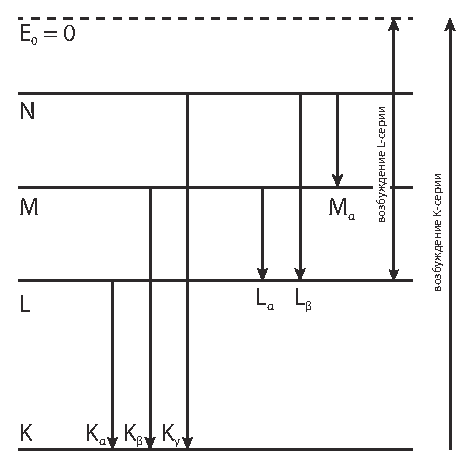
\includegraphics[width=.4\textwidth]{14_01} \hspace{1em}
    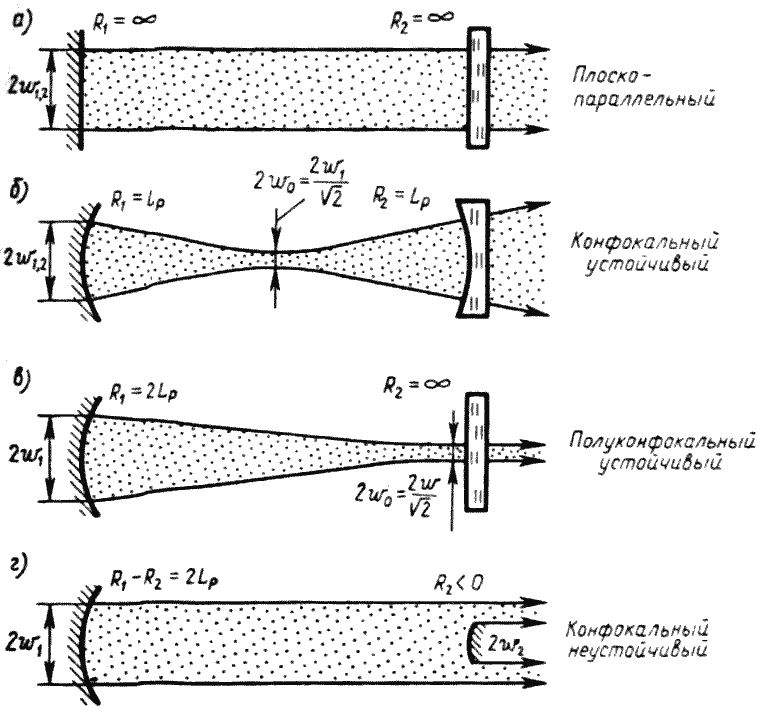
\includegraphics[width=.4\textwidth]{14_02} \\
    \parbox{.4\textwidth}{\caption{} \label{img14.1}} \hspace{1em}
    \parbox{.4\textwidth}{\caption{} \label{img14.2}}
\end{figure}

Добротность резонатора \( Q \) напрямую зависит от его свойств.
\[
    Q = \frac{2\pi W(t)}{W(t)-W(t+T)}
\]
